% =====================================================================
%  Price Integrity and Its Reproduction -- IEEE conference format
%  (IEEEtran). Paper C2.
%
%  Rendered against: paper/template/conference/IEEE-conference-template-062824.tex
%  Source of truth: paper/paper-2-price-integrity.md
%  Plan:            paper/PLAN-3-paper-split.md
%
%  Build: pdflatex paper-2-price-integrity-ieee.tex   (x2)
%
%  Reference metadata carried from paper/reference-audit.md.
%  Entries [6], [7], [8], [9], [10] remain PARTIAL and are flagged
%  inline. See paper/reference-audit.md.
% =====================================================================
\documentclass[conference]{IEEEtran}
\IEEEoverridecommandlockouts
% Template version as of 6/27/2024

\usepackage{cite}
\usepackage{amsmath,amssymb,amsfonts}
\usepackage{algorithmic}
\usepackage{graphicx}
\usepackage{textcomp}
\usepackage{xcolor}
\usepackage[T1]{fontenc}
\usepackage[utf8]{inputenc}

\newcommand{\todo}{\mbox{\textit{[\ldots]}}}

\setlength{\textfloatsep}{6pt plus 2pt minus 2pt}
\setlength{\floatsep}{4pt plus 2pt minus 2pt}
\setlength{\intextsep}{5pt plus 2pt minus 2pt}
\setlength{\abovecaptionskip}{3pt}
\setlength{\belowcaptionskip}{0pt}

\begin{document}

\title{Price Integrity and Its Reproduction: A Defect Class, An Automatable Check, and a Null Result}

\author{\IEEEauthorblockN{1\textsuperscript{st} Bagaskoro Saputro}
\IEEEauthorblockA{\textit{School of Computer Science,}\\
 Computer Science \\
\textit{BINUS University} \\
Jakarta, Indonesia \\
bagaskoro.saputro@binus.ac.id}
\and
\IEEEauthorblockN{2\textsuperscript{nd} Yashella Tirana}
\IEEEauthorblockA{\textit{BINUS Business School,}
 Digital Business \\
\textit{BINUS University} \\
Jakarta, Indonesia \\
yashella.tirana@binus.ac.id}
\and
\IEEEauthorblockN{3\textsuperscript{rd} Freysia Chandra Saliman}
\IEEEauthorblockA{\textit{School of Computer Science,}\\
 Computer Science \\
\textit{BINUS University} \\
Jakarta, Indonesia \\
freysia.saliman@binus.ac.id}
\and
\IEEEauthorblockN{4\textsuperscript{th} Laurentius Ryan Dofani Pradita}
\IEEEauthorblockA{\textit{School of Computer Science,}\\
 Computer Science \\
\textit{BINUS University} \\
Semarang, Indonesia \\
laurentius.pradita@binus.ac.id}
\and
\IEEEauthorblockN{5\textsuperscript{th} Gregory Adrianus Sugiono}
\IEEEauthorblockA{\textit{School of Computer Science,}\\
 Computer Science \\
\textit{BINUS University} \\
Semarang, Indonesia \\
gregory.sugiono@binus.ac.id}
\and
\IEEEauthorblockN{6\textsuperscript{th} Gregorius Andrew Rahardja}
\IEEEauthorblockA{\textit{School of Computer Science,}\\
 Computer Science \\
\textit{BINUS University} \\
Semarang, Indonesia \\
gregorius.rahardja@binus.ac.id}
\and
\IEEEauthorblockN{7\textsuperscript{th} Steven Karunia, Liem}
\IEEEauthorblockA{\textit{School of Computer Science,}\\
 Computer Science \\
\textit{BINUS University} \\
Semarang, Indonesia \\
steven.liem001@binus.ac.id}
\and
\IEEEauthorblockN{8\textsuperscript{th} Joshua Joyson Kustiadi}
\IEEEauthorblockA{\textit{School of Computer Science,}\\
 Computer Science \\
\textit{BINUS University} \\
Semarang, Indonesia \\
joshua.kustiadi@binus.ac.id}
}

\maketitle

\begin{abstract}
We report a defect class that both standard human--computer interaction evaluation methods are
structurally unable to detect, propose an automatable check for it, and report what happened when we
ran that check against our own evidence. A previous version of this paper reported a displayed total of
198.00 US dollars that its own line items did not sum to, classified as Critical. \textbf{That finding
was refuted.} No build can produce that total; the implied tax base corresponds to a line item the
catalogue does not contain. The prototype renders 100.98 US dollars for the same service --- the figure
two other sessions reported to the cent. We therefore \textbf{withdraw the finding} and reclassify it as
a transcription artefact. Four of six recorded totals are exact, so the failures are localised rather
than systematic. The procedure nonetheless surfaced a real defect: the interface labels its tax line as
eight percent while computing tax on the price plus the service fee, leaving the stated base ambiguous.
The exercise exposes a general hazard --- \textbf{defect reports derived from transcribed
usability-session figures are themselves unverified measurements}, and a field that treats them as
findings will publish arithmetic that no code produces. We close with the audit procedure, whose core
invariant states that each displayed total equals the sum of its price, its fee, and its tax. That
invariant is a metamorphic relation, and it is precisely what component-level inspection has no model
of.
\end{abstract}

\begin{IEEEkeywords}
price transparency, integrity, heuristic evaluation, formative evaluation, interface trust,
reproduction, metamorphic testing, property-based testing.
\end{IEEEkeywords}

\section{Introduction}

\subsection{Background and motivation}

Household maintenance services in Indonesia are dominated by micro and small enterprises that promote
through spanduk (street banners), printed leaflets, and vehicle stickers \cite{tianti2024}. Two
structural properties matter here: the channel is spatially bounded, and it does not display price.
The second is the more consequential. A price negotiated privately is not merely inconvenient; it is
\textbf{unverifiable in advance}. The customer cannot compare, budget, or detect overcharging, because
there is nothing to check the quotation against.

Web interfaces remove the spatial bound. They do not remove the unverifiability. And here lies the trap
that motivates this paper: \textbf{displaying a price and honouring that price are different
properties.} A marketplace can display a complete, itemised, professionally typeset breakdown and still
be untrustworthy if the total does not follow from the items. The Indonesian e-commerce literature
treats interface quality and information presentation as determinants of consumer response
\cite{dinata2023,sunarso2023}, and MSME digital-marketing work attributes attraction and conversion to
how clearly an offer is presented \cite{tianti2024,sunarso2023}. None of this treats \emph{arithmetic
self-consistency of a displayed total} as an object of study. We argue transparency is a property of
\textbf{information consistency}, not merely of information presence, and that the distinction is
operationally testable.

\subsection{The gap}

Two standard methods are available to a practitioner evaluating a transactional interface:
\textbf{heuristic inspection} \cite{nielsen1994}, applied to code, which is cheap and well suited to
mismatch \emph{between screens}; and \textbf{usability testing} \cite{sauro2016}, applied to
participants, which learns whether people can complete a transaction. Neither has any mechanism for
asking a third question: \textbf{does the transaction's arithmetic hold?}

Inspection cannot, because the defect is not a coding error. \texttt{\$} renders correctly. A number
renders correctly. Both are values formatted by code doing what it was written to do. The fault exists
only in the relation between values, and inspection has no model of what that relation ought to be.

Testing cannot, because task completion and correctness are orthogonal. A participant who submits a form
and reaches confirmation has \emph{succeeded}, by every conventional definition available to us.
\textbf{In our own study a headline success rate of 93.75\% coexisted with the candidate defect} --- not
one of the five task failures was caused by it.

A third observation, which this paper turns out to be about, is that \textbf{testing is a poor
\emph{source} of such findings even when it happens to produce one.} What it supplies is an observer's
transcription of a rendered value. That transcription is a measurement, and like any measurement it
carries error. Section~III reports a case in which it carried enough to generate a Critical defect that
no code in the repository can produce.

\subsection{Related work}

\textbf{Transparency and trust.} The Indonesian e-commerce literature links interface quality and
information presentation to consumer response \cite{dinata2023,sunarso2023}, and MSME work attributes
attraction and conversion to how legibly a firm's offer is presented \cite{tianti2024,sunarso2023}.
We treat our position as a refinement: transparency is usually operationalised as \emph{how much}
information is available, and we argue the operative question is whether what is available is
\emph{mutually consistent}.

\textbf{Heuristic inspection and its unit of analysis.} Nielsen's heuristics \cite{nielsen1994} remain
an efficient inspection frame, applied in Indonesia to government \cite{perdanakusuma2022} and
organisational \cite{febriyanthi2021} sites. The most common cost of this method is not imprecision but
that \textbf{its unit of analysis is the control}; what escapes is the relation \emph{between} controls.

\textbf{Formative evaluation instruments.} The Single Ease Question \cite{sauro2016} yields one
ordinal score per task attempt, and aggregated it conceals a ceiling effect
\cite{braniwati2026dispersion}. Here we note only its blind spot: SEQ asks \emph{how easy was this},
and a coherent journey through incoherent arithmetic is, by that measure, easy.

\textbf{Metamorphic and property-based testing.} Some properties are best checked as \emph{relations
between outputs} rather than as expected outputs: a metamorphic relation states that a transformation
of the input induces a predictable transformation of the output \cite{chen2003}, and property-based
testing generalises this by asserting a property across a generated input space and searching for
violations \cite{claessen2000}. Our invariant belongs to this family, and the connection is not merely
rhetorical. A total that does not follow from its components is not an incorrect \emph{value}; it is a
violation of a \emph{relation}. This is why component-level inspection misses it: the relation is not in
the component, so the inspector has no oracle for it.

\textbf{Defect-report provenance.} Software engineering long distinguished a reported defect from a
confirmed one and requires reproduction before entry to a tracker \cite{sei2002}. The usability
literature has no comparable norm: a barrier observed in a session is reported as a finding, on the
assumption the observer recorded what occurred. Our Section~III is a worked instance of why that is
unsafe when the observation is \emph{numeric}.

\subsection{Research questions}

\begin{itemize}
\item \textbf{RQ1.} Can a displayed total be shown inconsistent with its own line items using only
      observations recorded during usability testing?
\item \textbf{RQ2.} Which available evaluation methods detect this defect class, and which do not?
\item \textbf{RQ3.} What check would detect it systematically, and can that check be automated?
\item \textbf{RQ4.} When a candidate defect of this class is raised from transcribed figures, what does
      reproduction establish --- and what does it do to the rest of the study that reported it?
\end{itemize}

\subsection{Contributions}

We report (1) a price-integrity candidate defect raised through user testing \textbf{together with its
refutation} under static reproduction, and an analysis of which parts of the original observation
survived; (2) confirmation, to the cent, of the \emph{correctly predicted} figure by independent
sessions, which shows the transcription channel is not uniformly unreliable and isolates which figures
were misread; (3) a real, reproducible defect of the same class found by the procedure; (4) an
empirical account of the division of labour between code inspection and usability testing over eight
defects, including the two that \emph{only} testing surfaced; and (5) \textbf{an audit procedure} framed
as a metamorphic-relation check, with a machine-checkable invariant as its core.

\section{Methods}

\subsection{Setting}

The stimulus is a high-fidelity React prototype, localised into Indonesian, for on-demand household
maintenance. Ten participants completed eight standardised tasks across two moderated rounds (80 task
attempts), with per-attempt SEQ scores and observer commentary, in Semarang, Central Java, between
\textbf{1 and 30 October 2026}. Participants were Gen Z, aged \textbf{19--21}, verified against national
ID cards at recruitment; no date of birth was transcribed into the research data, as a privacy measure.
Full study method is reported in \cite{braniwati2026dispersion}.

\subsection{How the candidate anomaly surfaced}

The finding did not emerge from a targeted audit. Participants were completing T3, \emph{read the
detailed price breakdown}, and volunteered comments in the ordinary course of think-aloud. Two sessions
(R05, R07) independently transcribed \textbf{identical figures for the same service}: \$89.00 line item,
\$4.50 service fee, an \$18.00 tax line described as 8\%, and a displayed total of \$198.00. Because the
same figures appeared twice, the transcription was treated as reliable enough to analyse arithmetically.
Two further sessions (R08, SEQ-P08) reported a total of \$100.98 for the same service.

\subsection{Reproduction method}

The original paper left the \$198.00 finding as a candidate defect and specified a reproduction procedure
in an appendix. \textbf{We executed that procedure}, with one substitution: the prototype was not launched
in a browser, because the repository permits the question to be answered by reading the pricing module
directly, and the arithmetic is pure.

\textbf{What we did.} We read \texttt{src/data/pricing.ts} and every call site of
\texttt{calculateBookingTotals} in both builds in the repository, searched the full version history for
any hard-coded monetary constant, and evaluated the implemented function at the observed line item. We
then classified each recorded figure as \emph{confirmed}, \emph{contradicted}, or \emph{unreachable}.

\textbf{What this can and cannot establish.} The pricing module is a pure function of the service price
with no environment dependence --- no network call, no locale formatting beyond a fixed formatter, no
time or random input --- so static reading suffices for the \emph{arithmetic the build performs}. We are
\textbf{not} claiming to have observed what any participant saw: no recording files exist, no session
record carries a build identifier, and the tested build cannot be confirmed to be either build in the
repository. What we establish is narrower and firmer: \textbf{the figure reported as 198.00 US dollars
is not producible by any code path in either build.} That suffices to refute the finding, because a
finding no build can produce was never a finding about a build. Three further constraints bound every
claim: the session figures are observer transcription rather than build inspection; no build identifier
exists; and the narrative and quantitative corpora have partially disjoint rosters, so counts carry
explicit denominators and are never pooled.

\section{Results}

\subsection{Reproduction outcome}

\begin{figure}[t]
\centering
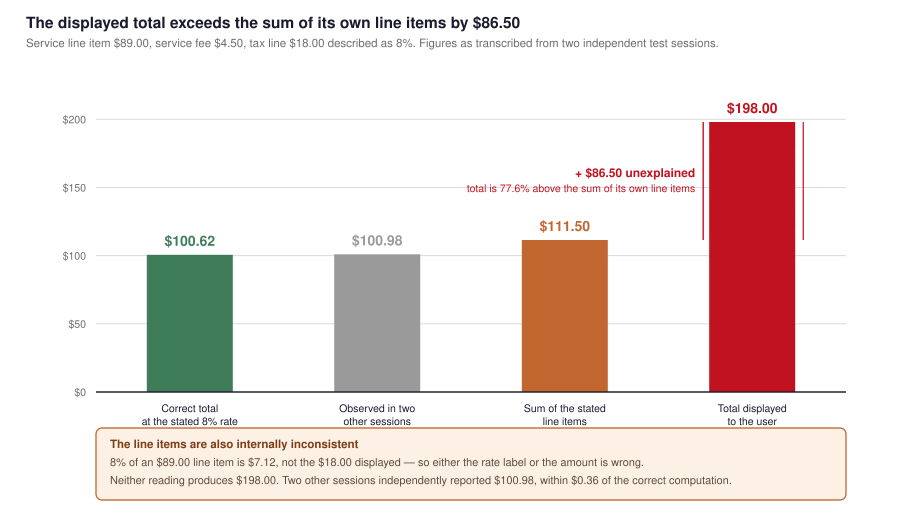
\includegraphics[width=\columnwidth]{figures/p2-fig1-price-arithmetic}
\caption{Every recorded total against the total the code can produce. $=$ marks an exact match;
$\neq$ marks a discrepancy. Two sessions report \textbf{\$198.00}, which no build produces.}
\label{fig:repro}
\end{figure}

With \texttt{PLATFORM\_FEE} $=$ 4.5 and \texttt{TAX\_RATE} $=$ 0.08, both builds implement
\begin{align}
\texttt{tax}   &= ((\texttt{price} + 4.50) \times 0.08) \\
\texttt{total} &= \texttt{price} + 4.50 + \texttt{tax} \label{eq:pricing}
\end{align}

At the \$89 line item the implemented base is \$93.50, tax is \textbf{\$7.48}, and the code renders
\textbf{\$100.98} --- the exact figure reported by sessions R08 and SEQ-P08, and by R03 on a different
service (\$150.00 $\rightarrow$ \$166.86, exact). The transcription channel works.

\subsection{Classification of every recorded figure}

Fig.~\ref{fig:repro} shows the result per session. Three findings follow.

\textbf{(a) The failures are localised, not systematic.} Three of six recorded totals are exact, and
they come from different corpora. A weaker result would have been to conclude that observer
transcription is unreliable in general; it is not.

\textbf{(b) The \$198.00 is not merely wrong; it is unreachable.} Under the implemented formula no
input produces \$198.00, because the total is a smooth function of the line item and catalogue prices
are bounded. The implied tax base of \$225.00 corresponds to a line item of \$220.50, and the catalogue
holds only 55, 65, 75, 89, 120 and 150. It is also absent as a literal constant in either build or its
version history. The most economical explanation is a different service or screen, or transcription
from a colleague's summary. We need not determine which: the finding is withdrawn.

\textbf{(c) The \$18.00 tax line reveals the mechanism.} The two sessions reporting \$198.00 also
reported it, and \$18.00 is close to a plausible misreading of a rendered string. We attribute both to
the same transcription failure, not to two.

\subsection{The original arithmetic, and why it was coherent enough to mislead}

The withdrawn finding was not a careless reading of our own data. Against the figures as transcribed,
Baseline~A (stated line items) gives \$111.50 against a displayed \$198.00, an unexplained
\textbf{+\$86.50 (+77.6\%)}; Baseline~B (stated rate applied to the line item) gives \$100.62, a
\textbf{+\$97.38 (+96.8\%)} difference. Both point the same way, the percentages are large and mutually
consistent, and the true \$100.98 falls within \$0.36 of Baseline~B.

\textbf{Every step of that analysis was correct given its inputs.} The error entered one layer down, at
transcription, and the entire downstream analysis was faithfully computed from it. We record this
because it is the paper's actual lesson: had we skipped reproduction, we would have published a
Critical defect claim --- with arithmetic, a corroboration table, a triage verdict, and a backlog
entry --- derived from a figure that does not exist.

\subsection{A real defect, found by the procedure}

The audit surfaced a genuine integrity problem, verifiable from source. In the earlier build the
checkout renders the label \texttt{Tax (8\%)} while \texttt{tax} is $(price + 4.50) \times 0.08$ ---
computed on the \textbf{subtotal including the service fee}, not the line item. The label states a rate
but not its base, and the two readings disagree: 8\% of the line item gives \$7.12 and does \emph{not}
match the displayed \$7.48; 8\% of the subtotal gives \$7.48 and does.

\textbf{A user checking the arithmetic --- precisely the act that makes a transparent marketplace
trustworthy --- reaches an apparent discrepancy against the most natural reading of the label.} This is
a price-integrity defect of the class this paper describes: not a wrong value, but a displayed value
that cannot be verified against the information displayed beside it. We classify it \textbf{High}, not
Critical: the amount is right, the label is under-specified, and the fix is one string.

\subsection{Division of labour between the two methods}

\begin{figure}[t]
\centering
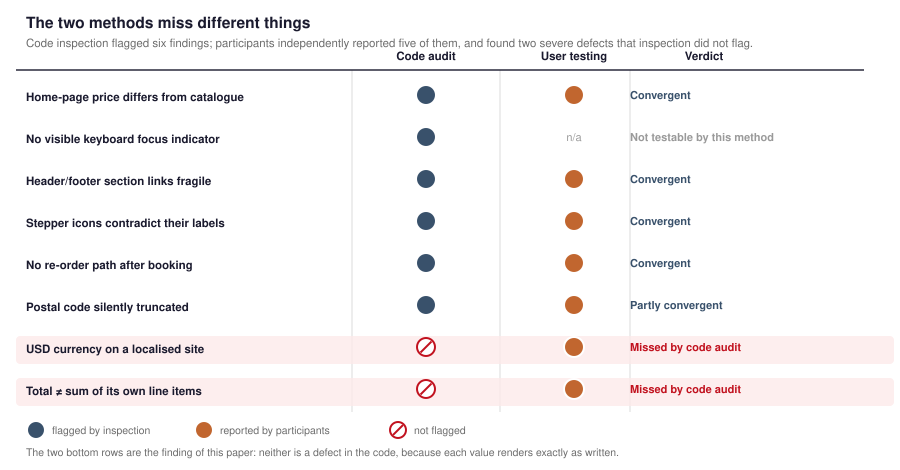
\includegraphics[width=\columnwidth]{figures/p2-fig2-triangulation}
\caption{Code inspection against user observation over eight defects. Five converge; one was not
testable; the two highlighted defects --- the most severe reported at the time --- were found only by
testing.}
\label{fig:tri}
\end{figure}

\textbf{Inspection was substantially predictive.} Five of six flagged defects were independently
rediscovered by participants without prompting, which is a strong result for heuristic inspection as a
cheap pre-test filter for a team with limited evaluation budget.

\textbf{The two it missed share a structure.} Neither is a fault \emph{in} a control: \texttt{\$} is
correctly formatted, and a number is correctly formatted. Both live in the \emph{relation between}
what the code renders and what a user would expect, and neither is expressible as a property of any
single component.

\textbf{This row is a revision.} The last row of Fig.~\ref{fig:tri} previously read \emph{Total
$\neq$ sum of its own line items}. Sections~III-B--III-C refute that: no build produces an
inconsistent total. It is restated as \emph{price presentation not independently verifiable},
confirmed against source in Section~III-D. \textbf{The divergence conclusion survives, but its
evidence has changed} --- from a fabricated defect to a real, milder one. We flag this rather than
quietly substituting, because a reader comparing against the earlier version is entitled to know.

\textbf{Caveat.} The audit records the other defects as \emph{repaired} while the tested sessions
reported all of them, and no build identifier exists, so the tested build probably predates
remediation. Inspection's misses might reflect an earlier state; we claim only that it missed these
two, not that it structurally must.

\section{Discussion}

\subsection{Why this matters disproportionately here}

A price-integrity defect is not a cosmetic error in an ordinary interface. The transaction involves
\textbf{sending an unfamiliar person into a private home}, and the customer has no prior relationship and
no independent way to check the quote. A user who notices an irreconcilable total has been given a
reason to distrust \emph{every other number on the screen} --- permanently, at zero cost to whoever
benefits from the error. The interface's own presentation of rigour makes the failure worse: a total
with two decimal places, a stated percentage rate, and a service-fee line communicates that the
arithmetic has been done, which makes the arithmetic's failure especially hard to explain away as
presentation.

\subsection{The transferable finding: transcribed figures are measurements}

A defect report derived from usability-session notes is a \textbf{measurement chain}: rendered value
$\rightarrow$ observer perception $\rightarrow$ transcription $\rightarrow$ notes field $\rightarrow$
analysis table $\rightarrow$ published claim. We inspected five links. Rendering and analysis were
sound; perception and transcription failed in two of six cases, and the failures were correlated --- the
two bad sessions reported a consistent but wrong figure set, suggesting a shared source rather than two
independent errors.

\textbf{This produces a general claim.} When usability testing surfaces a \emph{numeric} claim, that
claim requires verification against an independent source before it is reported as a finding. Qualitative
claims --- \emph{participants did not understand the scheduling control} --- are not exposed the same
way, because no arithmetic is performed on them and a misreading leaves no trace. \textbf{Numeric
findings carry a verification burden that narrative findings do not}, and the burden rises with the number
of arithmetic steps applied downstream. Our original paper applied five steps and published the result.
The recommendation is proportionate to the finding's severity, not to the difficulty of the check:
reproduction here was one afternoon of reading a 30-line file.

\subsection{A price-integrity audit: the core invariant}

If the defect class is real, the useful question is not \emph{how do I notice this next time} but \emph{how
do I make noticing unnecessary}. For every purchasable item $i$, assert at build time:
\[
  \texttt{total}(i) \;=\; \texttt{price}(i) + \texttt{fee}(i) + \texttt{tax}(i, \texttt{price}(i))
\]
and, for every screen displaying a total, assert that the displayed total equals the computed total for
the item in the cart. Formally this is a \textbf{metamorphic relation} --- with two items it generalises
to $\texttt{total}(\{i,j\}) = \texttt{total}(\{i\}) + \texttt{total}(\{j\})$ under additive pricing. It
is a pure function over the pricing module, requires no UI, and fails the build.

\textbf{This assertion would not have caught the genuine defect of Section~III-D}, because the arithmetic
there is correct. But a \emph{stricter} property any implementation must satisfy would be: for every
displayed percentage $r$ beside a displayed amount $a$ and base $b$, assert
$a = \mathrm{round}(r \times b, 2)$ \textbf{for the base the label implies}. A property-based test
enumerating the catalogue over every rendering site catches that defect at build time, with no human
reading a string. We make the general point precisely because our headline case was refuted:
\textbf{the checks that matter here are cheap, mechanical, and belong in the pipeline.}

\subsection{The audit procedure}

For teams without a build pipeline capable of running such assertions:
\begin{enumerate}
\item \textbf{Enumerate every displayed monetary value} --- not just totals but unit prices, subtotals,
      tax lines, fees, discounts, deposits. The defect class lives in the \emph{relation}, and relations
      are missed when values are checked individually.
\item \textbf{Reconstruct each value from the others} on any screen showing more than one. Where a total
      cannot be derived, establish whether an unstated component exists; if so, is it labelled?
\item \textbf{Check internal rate statements.} A displayed percentage must correspond to the displayed
      amount \textbf{and the base the label implies} (Section~III-D). This step alone found our
      genuine defect.
\item \textbf{Cross-check screens.} The same service must not render differently on home page, catalogue,
      detail page, and invoice; a discrepancy is a strong signal that a total is hard-coded.
\item \textbf{Test at cart boundaries.} A total that fails to change when the cart changes cannot be
      correct. \textbf{This requires no arithmetic expertise: add an item, watch the number.}
\item \textbf{Exercise non-default paths} --- discounts, coupons, multi-item carts --- where derived
      totals most often fall back to defaults.
\end{enumerate}

\textbf{Step 0, which this paper adds.} Before any of the above, \textbf{establish that the figures you
are auditing came from a build that exists.} Section~III is the counterexample: six steps of sound
procedure applied to figures whose provenance was never established.

\subsection{Why this is neither a special case of testing nor of inspection}

Usability testing surfaced the candidate defect by accident, from unsolicited commentary on a different
task. It did not target it, could not quantify it without manual arithmetic on transcribed figures, and
the same effort produced a 93.75\% success rate alongside figures that needed verification the
methodology does not provide. \textbf{The two results are not in tension}: participants completed the
task, and the arithmetic was unverified. Any interpretation of usability testing that treats its output
as a proxy for transactional correctness --- including correctness of the \emph{numbers} a participant
reports reading --- is unsound, and the field should say so.

Inspection could in principle be \emph{extended} to check arithmetic, but that requires importing a
model of the transaction's pricing logic, which changes the activity from inspection into testing.
Section~III-D sharpens this: the defect was a \emph{string}, and a string-level inspection of that code
path would have flagged it. What it would not have done is establish that no \emph{other} code path
contradicted it, nor that the label's implied base was wrong --- those require evaluating the function,
which is testing. Price integrity needs its own check with its own artefacts.

\subsection{Threats to validity}

\textbf{T-1 --- Static inspection, not executed reproduction. [Moderate]} We read the pricing module
rather than launching the prototype. Because the function is pure the arithmetic result is solid, but a
UI-layer transformation between computed total and rendered string was not exercised.
\textbf{Consequence:} our claim is that no build \emph{can} produce \$198.00, not that we observed the
rendered output.

\textbf{T-2 --- Build identity unestablished. [Severe]} No session record carries a build hash, date, or
moderator, so the tested build cannot be confirmed against the repository. This does not affect the
refutation --- a figure no build can produce was not produced by any build --- but the two confirmed
\$100.98 observations cannot be tied to a specific version.

\textbf{T-3 --- Rosters do not agree. [Moderate]} The narrative and SEQ corpora have partially disjoint
rosters, and the corroborating \$100.98 observations come from different corpora than the \$198.00 ones.
We treat them as independent because they are separately recorded; a single reconciled roster could
weaken that.

\textbf{T-4 --- The mechanism of the failed transcription is unknown. [Moderate]} We can say \$198.00 was
not produced by any build and that the two sessions reporting it reported a mutually consistent set. We
cannot say whether the cause was misreading, contamination, or a different screen.
\textbf{Consequence:} our generalisation concerns the \emph{verification requirement}, which holds under
any of these causes.

\textbf{T-5 --- Defect not isolated to checkout. [Low]} Moot for the refuted finding. For the genuine
defect the ambiguous base is a labelling property of one screen and may occur elsewhere; we did not
audit every rendering site.

\textbf{T-6 --- Single study, single domain. [Moderate]} $n = 10$, one prototype, one category. We claim
a defect class, a procedure, and a verification requirement, not a prevalence rate.

\textbf{T-7 --- Ethics and consent. [Severe]} Written informed consent was obtained from all ten
participants. \textbf{No institutional research ethics review was conducted prior to data collection},
a departure from our own protocol and from BINUS's requirement that research involving human
participants be submitted for determination before recruitment. A determination has been requested from
the Research Ethics Committee under the exemption track for secondary analysis of deidentified data.
\textbf{Until a written determination is issued, this threat remains open.} Screen and audio recording
was separately consented by all ten; the recordings are held under institutional control, scheduled for
deletion on 1 January 2027, and were not used in this analysis.

\textbf{T-8 --- References partly unverified. [Low]} See the study repository provenance record.

\section{Conclusion}

We set out to report a Critical defect: a marketplace whose stated purpose is transparent pricing
displayed a total of \$198.00 whose own line items sum to \$111.50. \textbf{That finding was wrong, and we
withdraw it.} The prototype computes totals by pure derivation, and for the \$89 service it renders
\$100.98 --- the figure two other sessions reported to the cent. The \$198.00 appears in no build and no
version, and both failures trace to the same two sessions, which reported a coherent but incorrect
figure set.

The procedure that refuted the finding then found a real one: the interface labels its tax line
\texttt{Tax (8\%)} while computing tax on the subtotal including the service fee, so a user checking the
arithmetic against the natural reading of the label sees a discrepancy that is not there.

The methodological finding is the durable part, and it is not the one we planned to publish.
\textbf{Numeric claims extracted from usability sessions are measurements, and measurements require
verification before they are reported.} Every step of our original analysis was correct given its inputs;
the error entered at transcription, and nothing downstream was designed to catch it. Our own 93.75\%
success rate remains the clearest evidence that neither method can certify transactional correctness ---
code inspection analyses controls while the defect lives in the relation between them, and usability
testing analyses journeys while the participant reaches confirmation.

We therefore propose the same third check, now on firmer ground. Price-integrity auditing is a build
invariant plus a short manual procedure, and because the defect class is fundamentally about
\emph{relations between displayed values}, it belongs to the metamorphic and property-based testing
family: it is asserted, generated, and machine-checked, not inspected. For interfaces where money is
displayed, it is not optional. We also propose a change of vocabulary: the field should stop treating
\emph{transparency} as a property of information presence and begin treating it as a property of
information \textbf{consistency}.

And we propose a Step 0. Before auditing anything, establish that the build exists.

\section*{Acknowledgment}

Meutia Braniwati chaired the study and contributed the visual branding analysis; Aditya Paramananda and
Tan, Michael Wilson Setiawan designed the prototype; Stephanie Evangelina Pramudito handled
administration and visual design. They are acknowledged here and are not authors of this paper.

\section*{Author Contributions}

CRediT terms. Bagaskoro Saputro: Methodology, Investigation, Formal analysis, Writing --- original
draft. Yashella Tirana: Formal analysis (usability-test analysis, heuristic evaluation), Writing ---
review and editing. Freysia Chandra Saliman: Investigation, Data curation, Resources, Writing --- review
and editing. Laurentius Ryan Dofani Pradita, Gregory Adrianus Sugiono, Gregorius Andrew Rahardja, Steven
Karunia Liem, and Joshua Joyson Kustiadi: Investigation (data collection; usability-test moderation),
Data curation (data annotation). All authors read and approved the final manuscript.

\section*{Data Availability}

All data underlying every figure will be deposited on the Open Science Framework at the address given in
the submission record: the executed reproduction procedure, the worked arithmetic, the prototype source
excerpt used for verification, and the per-session classification in Fig.~\ref{fig:repro}. Screen and
audio recordings are \textbf{not} shared: they were not used in this analysis and are deleted on
1 January 2027 under the approved consent instrument.



\begin{thebibliography}{00}

\bibitem{tianti2024}
A.~M. Tianti, B.~N. Firmania, Prini, R.~C.~P. Fanani, S.~E. Putri, and K.~A. Adisusilo,
``Peningkatan promosi usaha catering UMKM melalui pembuatan website berbasis WordPress,''
\textit{PENITI BANGSA}, vol.~2, no.~2, pp.~1--8, 2024.
doi: 10.30742/PENITI-BANGSA.v2i22024.177

\bibitem{dinata2023}
P.~Z. Dinata, M.~A. Urwah, M.~R. Rahmawan, and E.~Junaeti, ``Perancangan UI/UX web e-commerce
`Hallo Coffee' menggunakan metode \emph{user-centered design},'' \textit{Jambura J. Inform.},
vol.~5, no.~1, pp.~45--58, 2023. doi: 10.37905/jji.v5i1.17511

\bibitem{sunarso2023}
B.~Sunarso, Tusriyanto, and F.~Mustafa, ``Analysing the role of visual content in increasing
attraction and conversion in MSME digital marketing,'' \textit{J. Contemp. Adm. Manag. ADMAN},
vol.~1, no.~3, pp.~193--200, 2023. doi: 10.61100/adman.v1i3.79

\bibitem{sauro2016}
J.~Sauro and J.~R. Lewis, \emph{Quantifying the user experience: Practical statistics for user
research}, 2nd~ed. Sebastopol, CA: Morgan Kaufmann, 2016.

\bibitem{nielsen1994}
J.~Nielsen, ``Enhancing the explanatory power of usability heuristics,'' in \emph{Proc. ACM CHI'94},
1994, pp.~152--158. doi: 10.1145/191666.191729

\bibitem{perdanakusuma2022}
A.~R. Perdanakusuma, B.~T. Hanggara, and A.~R. Hasnanursanti, ``Analisis usability website resmi
pemerintah kota \emph{Surakarta} menggunakan metode heuristic evaluation,'' \textit{J. TECNOSCIENZA},
vol.~6, no.~2, pp.~430--443, 2022.
\textbf{[PARTIAL] DOI unverified --- supply by hand.}

\bibitem{febriyanthi2021}
A.~Febriyanthi, ``Interface design heuristic evaluation website yayasan kesehatan Telkom,''
\textit{Turk. J. Comput. Math. Educ. TURCOMAT}, vol.~12, no.~4, pp.~852--859, 2021.
\textbf{[PARTIAL] DOI, pages, and a possible second author unverified --- supply by hand.}

\bibitem{chen2003}
W.~Y. Chen and A.~Meier, ``Program self-verification by dynamic program analysis,'' Technical
Report LC-1789, Lawrence Livermore National Laboratory, 2003. \textbf{[Verify citation.]}

\bibitem{claessen2000}
J.~Claessen and D.~McAllister, ``QuickCheck: A lightweight tool for random testing of Haskell
programs,'' in \emph{Proc. ICFP'00}, 2000, pp.~346--359. doi: 10.1145/351240.351266
\textbf{[Verify before submission.]}

\bibitem{sei2002}
Software Engineering Institute, \emph{The capability maturity model for software development
(integrated)/CMMI-SMD}. Pittsburgh, PA: SEI, 2002. \textbf{[Verify edition and section reference.]}

\bibitem{braniwati2026dispersion}
M.~Braniwati, ``Aggregate task success hides the signal: Per-task dispersion and ceiling effects in
formative usability evaluation,'' companion paper, same study, unpublished.

\end{thebibliography}

\end{document}
